\documentclass[a4paper,12pt]{article}
\usepackage[utf8]{inputenc}
\usepackage[english]{babel}
\usepackage[pdftex]{graphicx}
\usepackage{anysize}
\usepackage{hyperref}
\providecommand{\keywords}[1]
{
  \small	
  \textbf{\textit{Keywords---}} #1
}

\title{Proyecto del curso: Latex y Git aplicado a la investigación científica}
\author{Elena Campoy}
\date{October 2019}
\marginsize{2.2cm}{2.2cm}{2.2cm}{2.2cm}
\begin{document}

\maketitle

\begin{abstract}
Inversions are a type of structural variation that has not been studied in detail due to their characteristics. Here I present some information about them: what they are, how are they formed, how can we detect them and some functional effects. In conclusion, as it has been difficult to deeply study them, we still do not know a lot about them. 
\end{abstract}

\keywords{Inversion, adaptation, InvFEST, clinical effects}

\section{Introduction}
A chromosomal inversion is a type of structural variant that consists of a change in orientation of a segment of DNA \cite{puig_human_2015, giner-delgado_evolutionary_2019}. It happens when a chromosome breaks at two points and the segment bounded by the breakpoints is reinserted in the reversed orientation \cite{kirkpatrick_how_2010}. In spite of being the first type of genetic variant to be studied and detected in {\em Drosohpila} \cite{kirkpatrick_how_2010}, some of their characteristics make its detection and study complicated. For example, they do not mean a gain or lose of genetic information \cite{giner-delgado_evolutionary_2019}. Therefore, they still remain as one of the most difficult classes of genetic variation to identify and characterize \cite{puig_determining_2019} and a bit of effort has to be done to fully understand their role in genetic variation. It has also been known for long that one of the main differences between our genome and others primates genomes is the presence of large chromosomal inversions. In figure 1 we can see the distribution of inversions between both genomes.
\begin{figure}[!htb]
    \centering
    \includegraphics[scale=1]{figures/inversions_hch.png}
    \caption{In this figure extracted from Kirkpatrick et al. 2010 \cite{kirkpatrick_how_2010} we can see the inversions that distinguish our genome and the chimpanzees }
    \label{fig:invchimpanzees}
\end{figure}
Appart from that, it is not clear how many polymorphic inversions really exist in humans and very little is known about their global frequency and distribution \cite{giner-delgado_evolutionary_2019}.



\subsection{Mechanism of formation}
We can distinguish two main types of mechanisms of inversion formation: NAHR: Non-Allelic Homologous Recombination (NAHR) and Non-Homologous End Joining (NHEJ):

\begin{itemize}
    \item {\bf NAHR:} 
    
    \
    This event occurs between sequences with high similarity in opposite orientation. Allelic Homologous Recombination (AHR) is a reparation mechanism of  double-stranded breaks (DSBs) in chromosomes by using the allele on the sister chromatid as a template. If this process occurs near a repeat, there can be some errors: the homology search could find a paralog of the repeat (instead of the sister chromatid) and NAHR is produced \cite{parks_detecting_2015}.
    
    \
    \item{\bf NHEJ:}
    
    \
    This is also a DSBs repair mechanism but it is not mediated by any repetitive element as it is a direct resealing of the DNA ends \cite{decottignies_alternative_2013}
\end{itemize}

In the figure 2 we can see a representation of both types of DNA repair mechanisms.
\begin{figure}[!htb]
    \centering
    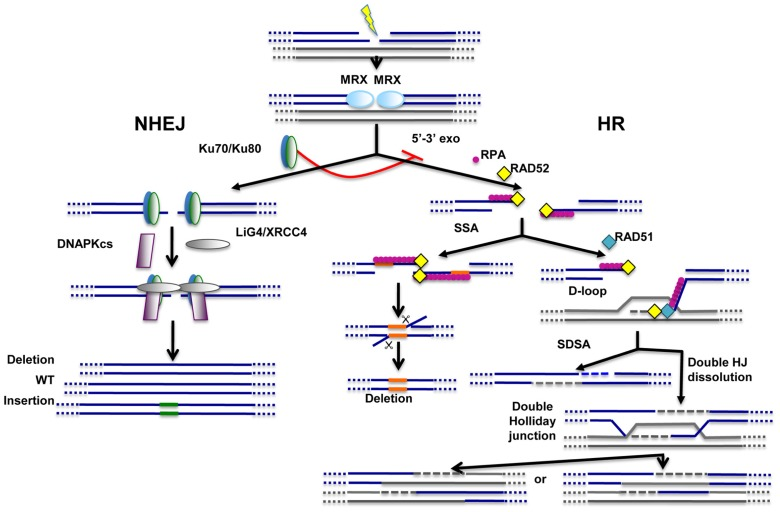
\includegraphics[scale=5]{figures/mechanisms.jpg}
    \caption{This figure \cite{decottignies_alternative_2013} represents both pathways to repair double-stranded breaks. We can observe NHEJ on the left and HR on the right}
    \label{fig:pathways}
\end{figure}

\
Other mechanisms that can induce the formation of inversions are: microhomology-mediated end joining (MMEJ), fork stalling and template switching (FoSTeS) or microhomology-mediated break-induced replication (MMBIR) \cite{vicente-salvador_detailed_2017}. 

\

As we can see, the type of mechanism by which the inversion is generated is related to the genome structure (the presence or absence of repeats) and it has also implications in the level of recurrence of an inversion. Normally, the inversions that occur through an event that is not related to genome structure have a low level of recurrence. In contrast, those that are present in a region that is prone to generate inversions through NAHR can happen more than once in a linage. It has been found a high-degree of recurrence of all inversions mediated by highly-identical inverted repeats (IRs) that could be rearrangement hotspots in the genome \cite{giner-delgado_evolutionary_2019}. 

\subsection{Data bases}
Efforts have been made in order to have a reliable structural variants data set. In this sense, the Database of Genomics Variants has included inversions in its catalogue \cite{puig_human_2015}. More recently, \href{http://invfestdb.uab.cat/}{InvFEST database} database has emerged as a human polymorphic inversion catalogue that provides refined breakpoint locations, associations with genes and SDs, plus data on experimental validation, population frequency, known functional effects and evolutionary history \cite{martinez-fundichely_invfest_2014}.


\section{How to detect an inversion}

At the beginning, the efforts to identify inversions were done with cytogenic techniques that only allowed the detection of variants of several megabases. Later, traditional molecular approaches were also applied to the detection of inversions but the result was the same: most of the detected inversions were large. At present, new sequencing techniques have provided us with new methods and applications that can be used in the inversion detection \cite{puig_human_2015}. 
Some of the methods that are being currently used are:

\begin{itemize}
\item {\bf Paired-end mapping (PEM):} 

\
This technique is based on sequencing technologies. First, the genomic DNA is fragmented into short segments (approximately less than 300 bp) and then both ends of each segments are sequenced. These reads are mapped to a reference genome and the differences in span size and orientation of the mapped reads in respect to the sample are analyzed as they can indicate the presence of a SV \cite{alkan_genome_2011, korbel_paired-end_2007, medvedev_computational_2009}. In more detail: we expect the reads to map into the reference genome with the same span and orientation as they had in the sample genome. A difference in span can reveal an insertion or a deletion in the sample genome and a difference in the orientation can reveal an inversion. In respect to inversions, we expect the orientation of the pair of reads in the reference genome to be +/-. An inversion may have occurred if the orientation is +/+ or -/-. 
PEM has some advantages over other methods. In first place, it increases the resolution of SV detection to the level of confirmation by PCR. Second, it does not need a preparation of a DNA library by cloning \cite{korbel_paired-end_2007}. On the other hand, this method is not comprehensive \cite{alkan_genome_2011} and the detection of a SV by PEM is limited if it is located in a region with multiple copies of highly similar and long repeats which makes the accurate prediction of the breakpoints difficult \cite{alkan_genome_2011, medvedev_computational_2009,korbel_paired-end_2007}. As well, the SV detection depends on the insert size: longer insert size allows the detection of larger events but shorter insert sizes allows a better detection of smaller events and a better localization (better resolution of breakpoints) \cite{medvedev_computational_2009}. Another difficulty is the reliance on unique mappings \cite{medvedev_computational_2009}.

\item {\bf Genome comparison.} 

\
{\em De novo} genome assembly has been essential in the construction of high quality reference genomes that has allowed numerous discoveries by genome comparison \cite{chin_phased_2016}. One of these applications is the discovery of structural variants. The limitations that are faced using this approach are related to the construction of the genome: how the DNA library is built (read size), the assembler that is used, the characteristics of the genome itself (its complexity and length) or the time and computing resources employed to built the genome \cite{baker_novo_2012}. To try to overcome this difficulties, distinct methods have been developed that allow the use of algorithms  to compare contigs to reference genomes

\item {\bf PacBio SMRT sequencing.} 

\
This technique – a 3rd generation sequencing platform- is capable of offering long reads lengths (up to 20  kb) that can span through repetitive elements and help to resolve complicated areas of the genome \cite{chin_phased_2016, jiao_benchmark_2013, rhoads_pacbio_2015}. In contrast to short reads (generated by 1st and 2nd generation DNA sequencers) that are 100-200 bp long \cite{jiao_benchmark_2013}, PacBio offers a medium length of 20 kb, with a maximum of 60 kb \cite{rhoads_pacbio_2015}. The longer lengths has several advantages as it allows the assembly of genomes that contain high repetitive DNA, to close gaps in genome assemblies, to phase analysis of DNA polymorphisms, to discover rare isoforms of highly conserved gene families and to identify rare gene alternative splicings \cite{jiao_benchmark_2013}.
\

PacBio SMRT implies ligating hairpin adapters to both ends of a double-stranded DNA molecule, creating single-stranded circular DNA. A single polymerase binds to either hairpin adaptor and starts the replication: after it replicates one strand it can continue replicating the other strand as a closed circle was created before. It happens multiple time and finally a continuous long read (CLR) is obtained which can be split to multiple reads \cite{rhoads_pacbio_2015}.
Some of its advantages are \cite{jiao_benchmark_2013}: it does not need PCR amplification, it is single molecule sequencing, it has shorter turn-around time and, as it has been mentioned before, it can produce very long reads. Nevertheless, some limitations are \cite{rhoads_pacbio_2015}: lower throughput (due to the failure to anchor a polymerase or the loading of more than one DNA molecule), higher error rate in the CLR and a higher cost per base.

\item {\bf Optical mapping.} 

\
This method allows the detection of bigger inversions than the methods previously described so it can be used in a complementary way. First, the DNA is digested by a nicking endonuclease that creates single-strand nicks that are repaired with fluorescent nucleotides. Then, the DNA is linearized in nanochannels and an imaged is created by a fuorescent microscopy. The final output is the optical map in which the restriction sites on each DNA molecule are observable. In a comparison of this map with an optical map based on the reference genome SVs can be detected \cite{besenbacher_novel_2015, chin_phased_2016}.
Optical mappings can overcome the difficulty of detecting large or complex SVs, being this the great contribution of the method. It has been demonstrated that, as whole Svs are easily contained in a single optical map, the larger an SV  is, the easier it is for the OMSV to detect it in a feasible and accurate way. This property makes optical mapping a great complement to the sequencing-based SV callers such as PE mapping that tends to be more accurate in the detection of smallers SVs \cite{li_omsv_2017}. Actually, optical mapping cannot detect balanced SVs like inversions if they are small and without a unique nick pattern \cite{mak_genome-wide_2016}.
\

Apart from the many advantages, this method has its own limitations and they are related to the generation of the optical map itself. First, the existence of false positives (false labels observed that are not true restrictions sites) or false negatives (true restriction sites that cannot be observed in the maps) because of non-specific enzymatic cuts or incomplete enzyme digestion, respectively. Second, the resolution of the imaging system (labels of close restriction sites can merge into a single label) and uncertainties in DNA measurements (sizing errors that are deviations between measured and actual distance between two restrictions sites due to DNA fragments that are not completely linearized). Third, the creation of “fragile sites” leading to double-stranded breaks because of neighboring nicking sites on opposite strands. Fourth, the requirement of a {\em de novo} assembly of the optical maps that makes the accuracy of the SVs calls to depend on the reliability of these procedures \cite{li_omsv_2017, mak_genome-wide_2016}. Fifth, there can be some inaccessible zones of the genome because of the lack of nicking sites for the nicking enzyme and finally, this technique does not offer single basepair resolution \cite{levy-sakin_genome_2019}.

\item {\bf Strand-seq method.}

\
This method is based on the orientation of DNA as it is capable of conserving the orientation of each DNA strand. To achieve this, BrdU is incorporated into nascent DNA strands during DNA replication in order to distinguish between parental and daughter strands. Later, during the library preparation, the BrdU strands are selectively removed so that only template strands are amplified and sequenced. Finally, the reads from the Strand-seq library are aligned to a reference genome, displaying the reads counts on ideograms for each chromosome. Each read is aligned to either the forward or reverse direction of the reference genome.  
\
Just as optical mapping, Stranq-seq method allows the identification of large SVs \cite{sanders_characterizing_2016}, so it is again a good complementary method to PEM. It has also other applications: it can multiplex hundreds of single cells and it can be used in order to discover rare cells in heterogeneous samples, study genetic mosaicism or explore genomic variants between demographics \cite{sanders_characterizing_2016}. It has allowed the characterization of variants from 1 kb to 4.5 Mb and new inversions that could not be previously described due to the presence of blocks of segmental duplications \cite{sanders_characterizing_2016}. On the contrary to optical mapping, its low sequence coverage limits the size of detectable variants: the smallest inversion detected was 17 kb. It can also limit the resolution of the breakpoint mapping. In respect to the methodology, another limitation is due to the incorporation of BrdU: not all the cells can incorporate it. Finally, the protocol turns out to be expensive due to the required multiple enzymatic and cleanup steps.

\item {\bf Multiplatform approach.} 

\
As it can be elucidated from the previous points, no method allows the identification of all the distinct types of SVs that the genome contains. For this reason, a multiplatform approach for the discovery of SVs has been proposed in order to define the full spectrum of human variation \cite{chaisson_multi-platform_2019}. Employing more than one detection algorithm results in a maximum sensitivity and specificity in SV discovery. Nevertheless, using all the available sequencing methods in a single study is not practical as it implies a high cost and work. Analyzing the trade-off between the cost and the sensitivity of a technique is essential to achieve the desired result \cite{chaisson_multi-platform_2019}. 
\end{itemize}


\section{What does an inversion do?}
Due to all the difficulties to study inversions, we still lack of information that could be useful to answer some questions like: are inversions responsible of some diseases? Are they under positive or negative natural selection? Do their frequencies change between populations?

\subsection{Clinical consequencies}
Most of the inversions do not have any phenotypic effect of clinical significance. Normally, they show differences in frequency in different human populations \cite{puig_human_2015}. 

\
However, some of them are related to some diseases caused by the disruption of one gene or by the alteration of a gene expression. Some of the inversions produce diseases in a recurrent way, such as in hemophilia A and Hunter syndrome \cite{puig_human_2015}. In the table below we can see some polymorphic inversions that have been associated to phenotypes or diseases:

\

\begin{table}[!htb] % [!htb] para que salga justo ahí que es donde quiero que salga
\centering
\begin{tabular}{|l|c|}
\hline
\multicolumn{1}{|c|}{\textbf{Inversion}} & \textbf{Effect}                                       \\ \hline
\multicolumn{1}{|c|}{HsInv0573}          & Neurodegenerative disorders: Alzheimer and Parkinson  \\ \hline
HsInv0501                                & Systemic lupus erythematosus and rheumatoid arthirtis \\ \hline
HsInv0786                                & Protection against asthma and obesity                 \\ \hline
HsInv0472                                & Wolf-Hirschhorn syndrome                              \\ \hline
HsInv0301                                & Williams-Beuren syndrome                              \\ \hline
HsInv0415                                & Sex reversal/male infertility                         \\ \hline
\end{tabular}
\begin{tablenotes}
\small
\item In this table we can see the effect that each inversion (left column) has. The name of each inversion is in reference to InvFEST database \cite{martinez-fundichely_invfest_2014}.
\end{tablenotes}
\end{table}

\
\subsection{Adaptative consequences}
Apart from the clinical effects, there are some effects -that still need further study- produced by inversions: they are related to fertility problems or they can promote complex intrachromosomal arrangements and translocations. 

\
A case that has been deeply studied is the 17q21.31 inversion (HsInv0573). It seems to be under positive selection in Europeans: the inverted haplotype (H2) reaches high frequencies (∼10–35\%). It has been noticed that  women carrying either one or two copies of the inversion tend to have more children. However, other studies show that the high frequency of this haplotype might be the result of a founder effect instead of a positive selection.  \cite{puig_human_2015}.
\newpage
\bibliographystyle{plain}
\bibliography{project.bib}
\end{document}

